\chapter{Implementation\label{chap:implementation}}
This chapter will discuss the technical specifications of the project and discuss the decisions that affected the process. I will also overview my workflow and iterative approach to the project. Last but not least, I will include and credit a list of third-party libraries that this framework makes use of.

\section{Development process}

In this section, I will outline how the work on my dissertation was conducted along with pointing out the pitfalls and making sure that the project remains fully functional.

\subsection{Project plan}

\begin{figure}[h]
    \centering
    \makebox[\textwidth][c]{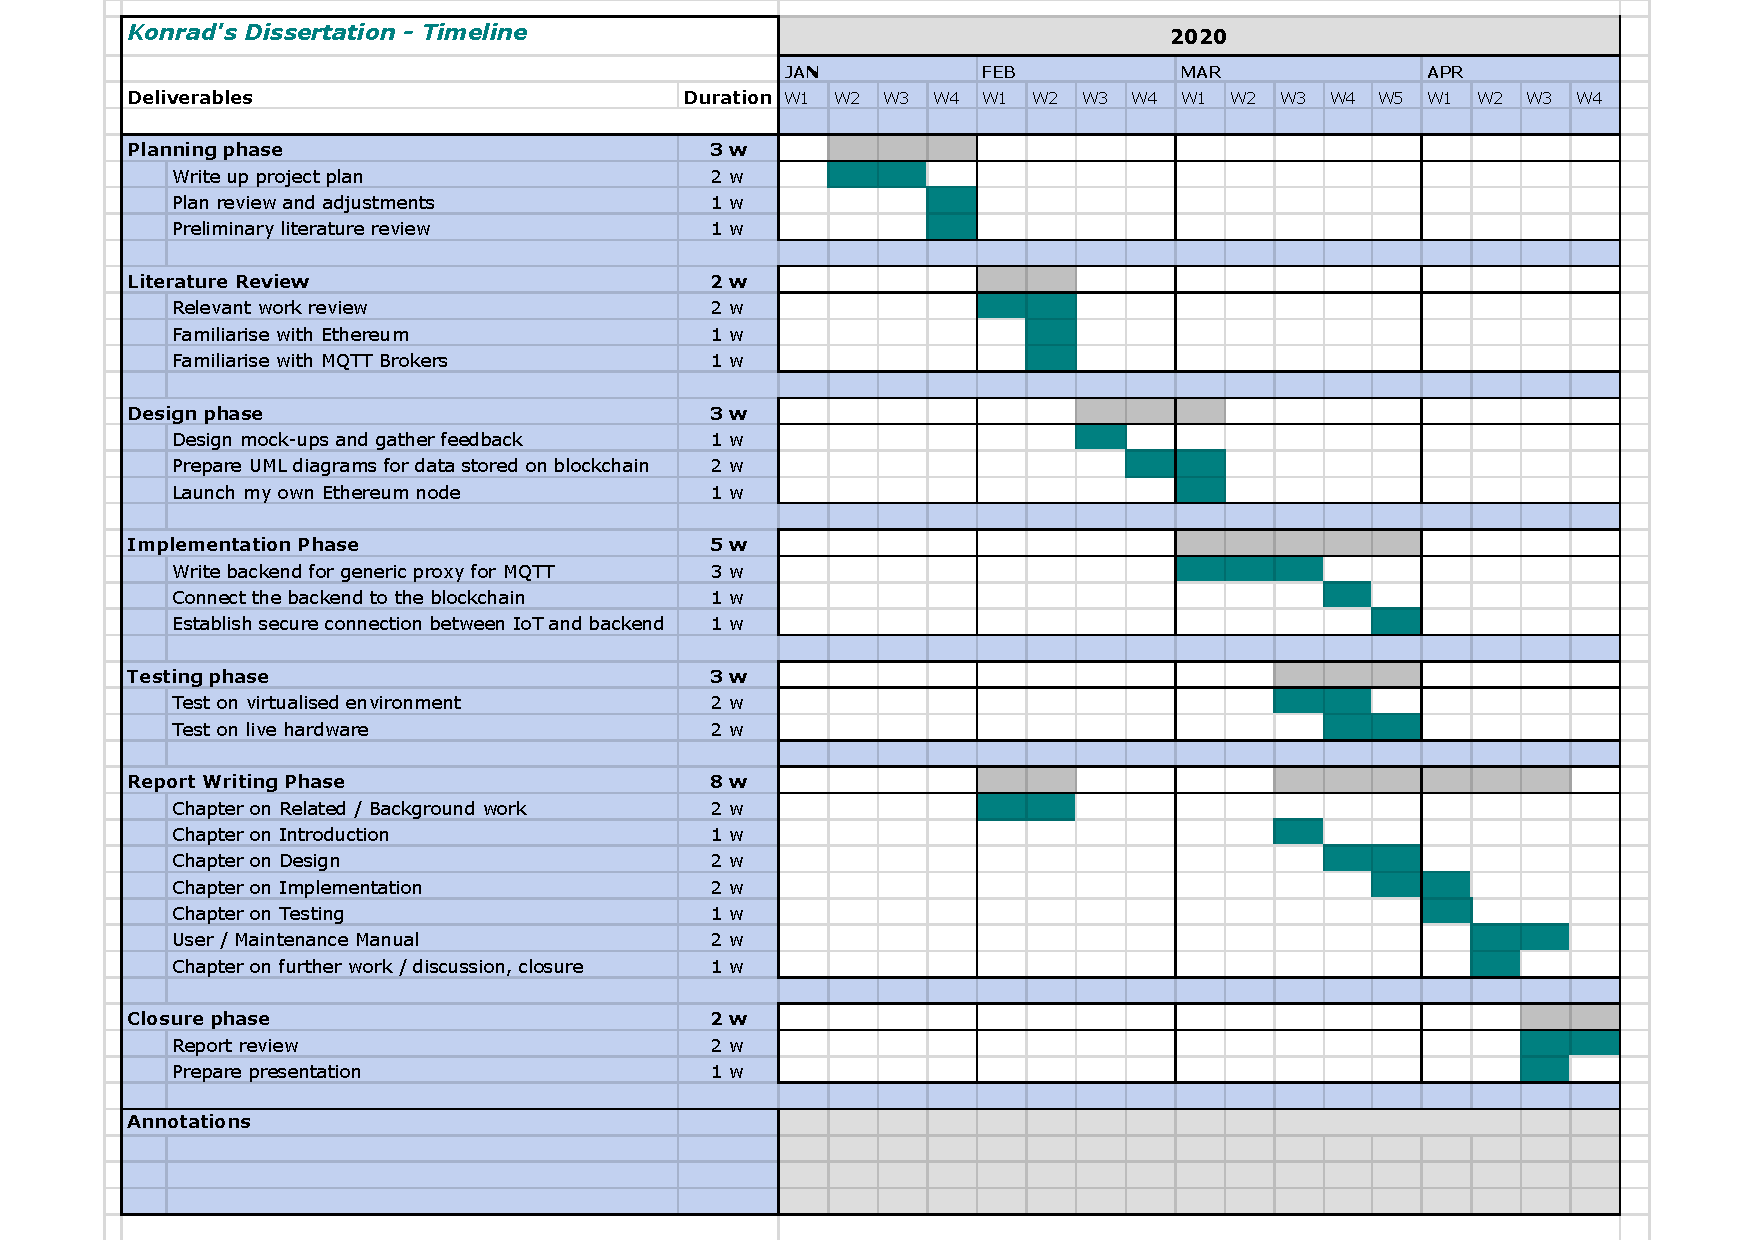
\includegraphics[width=1.1\textwidth]{timeline}}
    \caption{Project timeline}
    \label{fig:timeline}
\end{figure}

Figure \ref{fig:timeline} demonstrates the timeline of the project, and all included phases. Each of those tasks was also divided onto smaller subsections (not shown on the diagram), which were worked on using an agile approach, as described in the next paragraph.

\subsection{Iterative Approach}

When designing my project plan, I distributed the workload onto small chunks and features which would have been implemented iteratively. I was following agile methodologies, dedicating each week on a different feature, where I would go through the entire development cycle for each unit. For example, generating the reports (section 4.4.2) was first introduced during a meeting with my supervisor, where I would establish the requirements and success criteria for this particular story. Then I would spend a day or two designing the flow and functionality, followed by an extra two days implementing designed features. At the very end, I would conduct testing and regression testing to make sure that the rest of the project still remains operational. This would have been concluded with a meeting with my supervisor to reflect on the sprint and determine whether success criteria were met.

\subsection{Regression testing}

Since I was following an agile workflow when working on the project, it was essential to ensure that none of the `stories' (or, tasks) affected each other when completed. I could have found myself in a situation where working on the reporting of the events to the blockchain might have broken another, unrelated feature, e.g. verifying the authenticity of connecting clients. That is the reason behind keeping regression testing as a vital phase of development. I was able to achieve it through continuous, automated testing - which includes unit, integration, regression and manual testing.

\section{Technologies}

In this section, I will describe the technologies used in this project, that is, languages, frameworks, third-party libraries and different approaches when it comes to writing the code.

\subsection{Languages used}

Following programming languages have been used when working on this project:
\begin{itemize}
 \item \textbf{Golang} (v1.14) - main driver behind the proxy, MQTT client and for communicating with the blockchain. It has also be used in the backend for the web application.
 \item \textbf{Solidity} (v0.6.6) - language used to develop smart contracts on Ethereum.
 \item \textbf{HTML5 + CSS3 + JavaScript} - frontend stack used to create a simple website to display contents of blockchain.
\end{itemize}

\subsubsection{Golang}
Go (short for Golang) has been introduced in 2009 by Google \cite{team2009go}. It is a language which strongly follows parallel programming paradigms, allowing the developer to make use out of all available threads and cores to maximise the performance. Multi-thread performance was exceptionally sought after in this project, as FlyTrap is expected to handle many simultaneous proxy connections. In Golang, the programmer can make use of so-called goroutines, which the runtime can dynamically either place on separate cores or run them concurrently on the same core - depending on the task.

All Ethereum frameworks (such as go-ethereum or geth, explained further in section \ref{sec:tpp}) were also designed first in Golang. By deciding to write my project in Go as well, I ensured maximum compatibility, as I was able to use the official SDK's, rather than having to rely on unofficial solutions. I also was already experienced with Golang, as I spent a year in industry at Google working on several projects in that language, which decreased the learning overhead for my dissertation.

Go in the project was used to write the backend of the webserver, CLI to communicate with the blockchain and the proxy itself which handles all incoming connections.
\subsubsection{Solidity}
Solidity \cite{dannen2017introducing} is the language used to write smart-contracts in Ethereum, so unfortunately it was a necessity. Its syntax is similar to Javascript, though it is statically, strongly typed. go-ethereum includes a utility which translates Solidity code into Golang methods, which then can be used to make calls against the blockchain. There is no API which can be used to query/create transactions and rather developers need to use official SDKs published by Ethereum team.
\subsubsection{HTLM5 + CSS3 + JavaScript}
Since the web application serves only as a presentation and demonstration, I decided against any complex JavaScript or TypeScript frameworks and rather opted for a simple solution consisting of plain HTML + CSS and JavaScript. The web app also includes a small backend; thus, asynchronous calls are performed from the client-side towards the server to fill the content tables dynamically.
\subsubsection{Considered alternatives}
Apart from Golang, I was also considering \textbf{Python} as a main driver for the project. Majority of my projects in the past included Python, and my familiarity was sufficient to avoid any roadblocks. Though, compared to Golang, there are several problems, which would be especially prominent in this project, one of them being Global Interpreter Lock\cite{beazley2010understanding} (or GIL for short), which effectively restricts the scope of possible multithreading.

The choice was also dictated by a personal preference, as I wanted to apply the knowledge I gained over my year in industry during my final year at University. I believed that having a comparison on how a language performs in both industrial and academic environment might provide invaluable experience.
\subsection{Third party libraries \& resources}\label{sec:tpp}
Following resources - which I was not the author of - were utilised in the project. All of them include an open-source license, allowing unrestricted, free use (fulfilling \textbf{NFR4}):
\begin{description}
  \item[ethereum/go-ethereum v1.9.10] \cite{ethereum2017official} - official Go implementation of Ethereum blockchain used as a bridge between ETH nodes and any Golang programs, allowing to perform CRUD\footnote{Create, Read, Update, Delete} operations on the blockchain.
    \item[eclipse/paho.golang v0.9.1] \cite{pahogolang} - library used to unpack MQTT packets in Golang, without having to inspect each individual byte manually. It outputs a struct containing all fields as defined by MQTT v5.0 specification.
    \item[oschwald/geoip2-golang v1.4.0] \cite{geoip2} - coupled together with GeoLite2 IP Geolocation dataset from MaxMind \cite{maxmind} is used to determine the country in which the IP is located in, without having to query external APIs. 
    \item[tabulator v4.4.3] \cite{tabulator} - JavaScript library used to create dynamic data tables, which can be asynchronously populated and filtered on the client-side.
\end{description}

\subsection{Working with MQTT}
As the project heavily relies on MQTT brokers, I had to look for a solution to simulate this environment on my machine. I had two  options, either run the broker locally or use one of the publicly available test brokers
\subsubsection{Online Broker}
Both HiveMQ\footnote{https://www.hivemq.com/} and Mosquitto\footnote{https://test.mosquitto.org/} provide free, publicly available brokers capable of both TLS and plain TCP connections. Connecting FlyTrap to a live, online broker helped me test how would the system behave in a situation where FlyTrap and the broker are not located on the same machine and whether inter-network proxy works fine.
\subsubsection{Local Broker}
For maximised performance, local broker should be used, to minimise the latency of TCP/TLS connections. For that, I have used Mosquitto 1.6.9\footnote{https://mosquitto.org/blog/2020/02/version-1-6-9-released/}. I was also able to generate a new set of certificates and RSA public/private key pair for TLS connections\footnote{through `openssl' utility}.  
\subsection{Working with Blockchain}
Ethereum was to be used as a data layer for the application. Of course, testing on the public chain was out of the question, due to the tremendous costs involved. Fortunately, Ethereum provides an easy way to start your own network, which would behave identically as the real one (including fake credits to use) - in the end, it would be indistinguishable from the real node for the applications attempting communication. When working on the project, I considered two ways of mocking the blockchain and in the end, made sure to test FlyTrap in all two approaches:
\subsubsection{Ganache}
Ganache\cite{lee2019testing} is a framework designated for emulating Ethereum environment. It can be thought as a sandbox environment, where you can generate any required number of dummy accounts, preloaded with currency, which then can be used to transact with each other - all running on localhost, without the need of configuring a proper blockchain network. Extra blocks are mined automatically - as needed. It is also possible to dump the workspace into a file and check into version control.

Figure \ref{fig:ganache} shows how the interface looks like. You can generate as many wallets as possible, each with public/private key pair and preloaded with 100 ETH.
\begin{figure}[h]
    \centering
    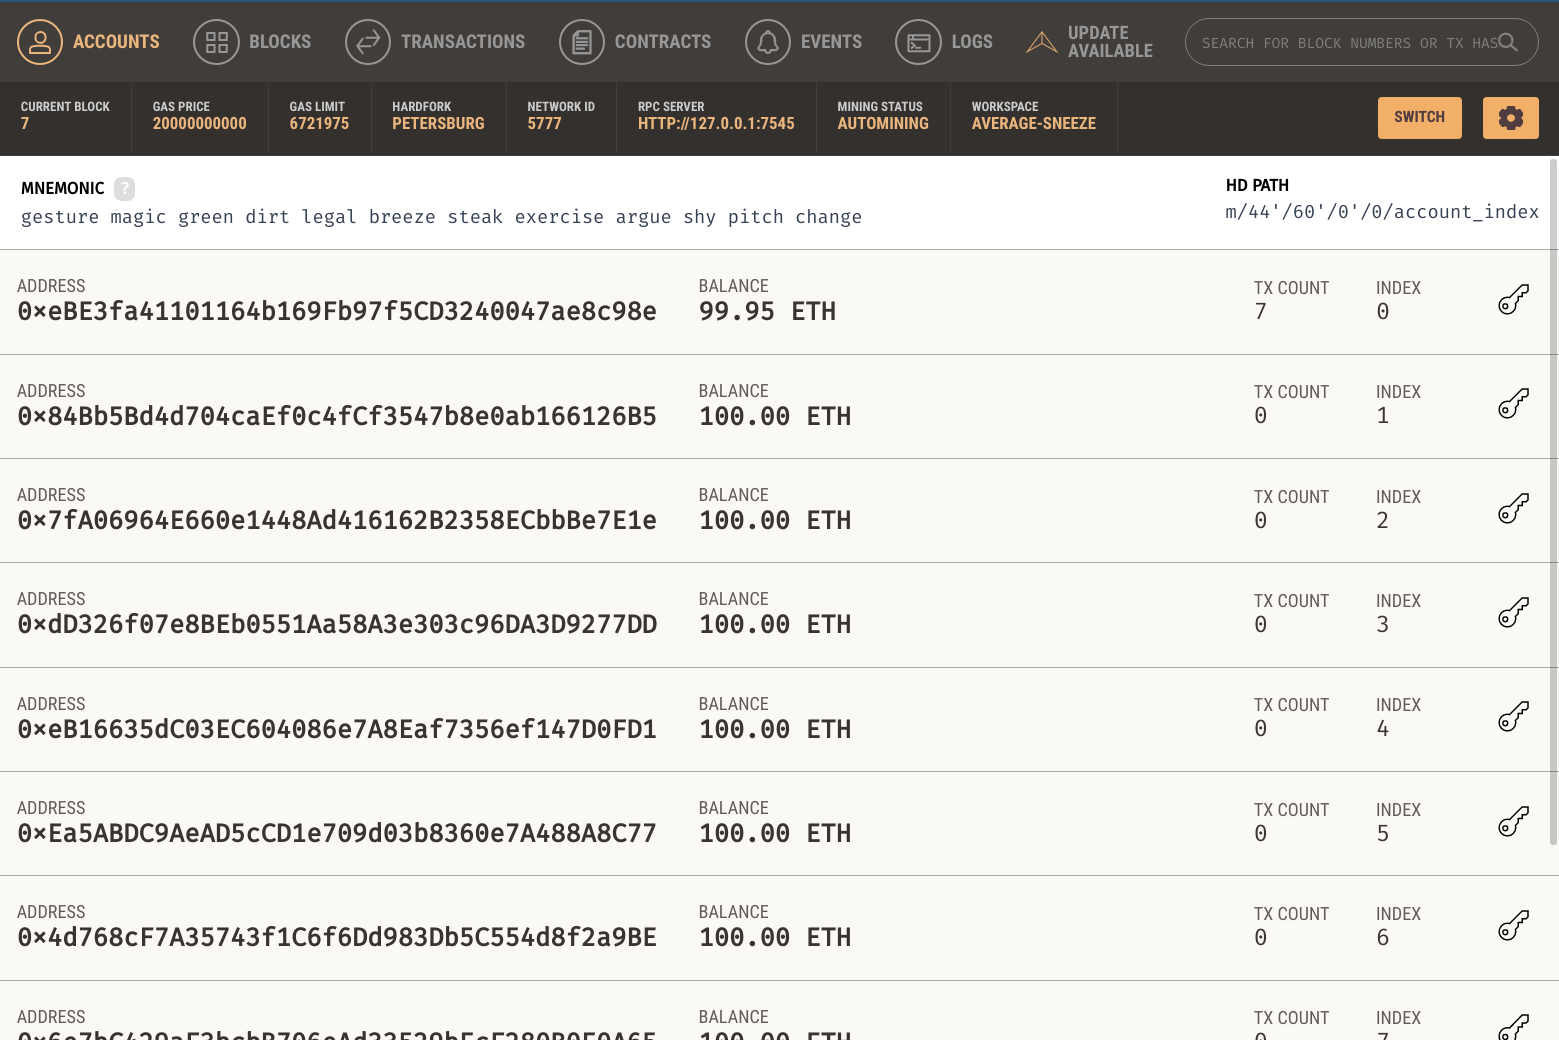
\includegraphics[width=0.9\textwidth]{ganache}
    \caption{Ganache Interface}
    \label{fig:ganache}
\end{figure}

\subsubsection{Geth}
Geth is an environment much closer to the real Ethereum node. In fact, it is a real Ethereum node. Geth is also used in production environments to set up new networks or nodes. When testing my framework, I have set up a new Proof-of-Authority network, with only one node. Since I am in control of the network, I can configure all parameters, such as cost of gas (decreasing it down to 0), allowed accounts or speed of mining new blocks. This network is also indistinguishable from a public one, similar to Ganache. Geth can also be used to connect to live networks and start mining cryptocurrency on your workstation.
%\subsection{Development tools}
%\hl{optional, get back here if i still have some wordcount left}
%\subsubsection{Version Control}
%\subsubsection{Text Editor}

\subsection{Configuration}
Application involves a lot of configurable values, to ensure that the end-user finds their preferred combination of settings (such as TLS certs, ports - see User Manual for an overview of all possibilities). There are several ways to state constants and parameters when running any of the components:
\begin{itemize}
    \item Command line parameters - to specify the environment when running the binaries.
    \item Environmental Variables - alternative to command line parameters. FlyTrap will first inspect command line parameters and if not, will look for environmental variables defined by the host OS.
    \item Constants in the code - for some immutable values, that do not require intervention (though the option to change them remains documented).
    \item Website requests - for the web application that ships alongside the project, user can also specify fields such as contract address or on which port Ethereum node is running under.
    \item Static files at projects root - since FlyTrap requires some user-provided files (such as private keys or certificates), running the proxy will require providing a path to those files via one of the methods specified above.
\end{itemize}
\subsection{Logging}
All significant operations on FlyTrap, Blockchain CLI and Web Backend are logged to standard error through log Golang module\footnote{https://golang.org/pkg/log/}. These logs are only produced only for primary operations such as new connection or any actions resulting in writing to the blockchain.

They are not persistent and will disappear upon restart. Users are free to implement their own redirection to local files if desired.

